\chapter{TonePrint}
\label{TonePrintConcept}

This chapter works as a in depth description of the TonePrint Concept. This information in this chapter could be essential to understand the later thoughts and considerations, regarding the development of a TonePrint community.

\section{What is TonePrint?}
\label{WhatIsTonePrint}

Effect pedals is a normal piece of equipment used by guitarists and bassists, in many different music genres. An effect pedal works by changing the input signal from the instrument, accordingly to the effect type. This gives the musician the ability to change the sound of the his/hers instrument, with a simple stomp on a box on the floor. By using normal effect pedals, you're normally limited in the sens of only being able to adjust a small number of parameters on physical knobs on the pedal. A simple guitar pedal is shown on \autoref{fig:EffectPedalExample}. On this example there is three separately adjustable parameters on the pedal (Dwell, Mix and Tone), which each have its own knob.

\begin{figure}
	\centering
	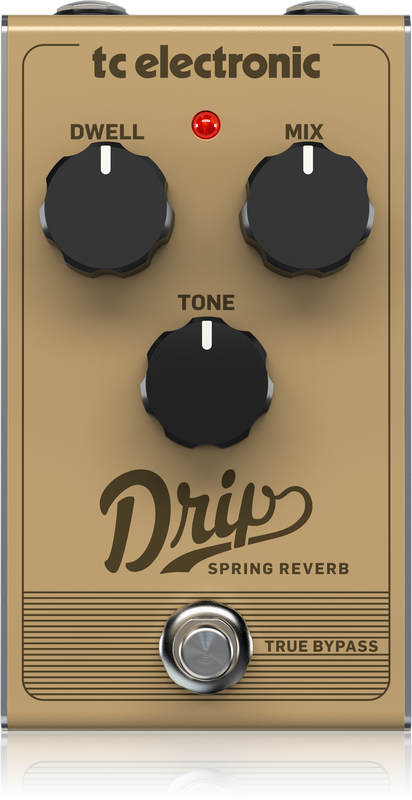
\includegraphics[width=.25\textwidth]{Graphics/EffectPedalExample}
	 \caption{This figure shows a Drip spring reverb effect pedal by TC Electronics.
    \label{fig:EffectPedalExample}
\end{figure}
 %https://www.tcelectronic.com/Categories/Tcelectronic/Guitar/Stompboxes/DRIP-SPRING-REVERB/p/P0CQ2#googtrans(en|en)

%\begin{figure}[H]
%	\centering
%	\includegraphics[resolution=300,scale=1]{}
%	\caption{}
%	\label{fig:}
%\end{figure}
%\noindent



%In 2011 TC Electronic revealed their first TonePrint pedals, opening a new playground for musicians and tone tweakers. By applying the smartphone as tool for setting the desired parameters for an effect type, the user can beam a preset from his or her smartphone directly to the pedal holding the effect type in question. The number of parameters varies between pedal types, and each setting of these parameters is what is simply referred to as \textit{TonePrints} \parencite{WEB:AboutTonePrints}.

%TC Electronic's application holds multiple templates made in-house with different effect types and styles, but it also holds multiple TonePrints created in collaboration with famous guitarists. These presets are referred to as \textit{Artist TonePrints}, and the expectation is that the user will have a clear expectation of the sound of the TonePrint, when it comes from his or her favourite guitarist \parencite[][8]{PDF:TonePrintAnalyse}. As such, the user has the option of either using a specific effect type as a starting point or having the desire of matching the sound of a famous guitarist. In either case the TonePrint is beamed to the effect pedal in question, allowing for further tweaking of the sound before it is send through the rest of the setup and perceived from the speaker. The user may also want to explore TonePrints from guitarists unknown to them and maybe influence his or hers way of playing \parencite[][8]{PDF:TonePrintAnalyse}.

%Despite the various templates and artist TonePrints, the motivation of the users may also be to develop their own unique sound from scratch, these presets are referred to as \textit{User TonePrints}. The user also manages these in the TonePrint app, but at its current stage these TonePrints are still constrained to reside in the user's app without a straightforward way of sharing the settings with other guitarists. The next step for the TonePrint concept therefore seems to be a community in some form, allowing users to share their unique TonePrints with each other.

%Det ovenstående afsnit børe dummes ned så det kan forståes af folk som ikke er guitarister eller kender til TC's produkter.
%TonePrint Editoren skal også beskrives.
%Nogle billeder og eksempler ville ikke være dumt.
%Hvis det ikke skal stå i introduktionen kan vi også komme mere i dybten med det. TonePrint er en vigtig del i vores opgave da det er dem som brugerne skal dele.


%Hvad skal der med i afsnittet om TonePrints?
%- Et unikt preset af en effekttype
%	- Disse effekttyper er tilknyttet deres egne pedaler, hvor TonePrints er forskellige indstillinger af disse effekttyper
%	- (Indstillingerne af effekten omfatter 50 - 100 parametre, afhængigt af pedal model)
%	- Pedalerne kan have mange forskellige TonePrints tilhørende sig, disse er skabt og tilpasset i samarbejde med stjerneguitarister
%- Intentionen med at lave TonePrints i samarbejde med kendte guitarister er at give brugeren en klar ide om, hvad de kan forvente af disse presets.
%	- En brugers udgangspunkt vil måske også være at lyde som sit absolutte idol.
%	- Alternativt, kan man også opdage TonePrints fra guitarister, hvis stil man ikke kender, og på den måde få udvidet sin horisont.


%		- Forventningsbekræftende vs forventningsbrydende
%	- TC's række af samarbejdspartnere er stødt stigende
%- Artist TonePrints vs User TonePrints
%	- Efter, man har taget udgangspunkt i et TonePrint, kan man foretage yderligere ændringer af det og på den måde gøre det til sit eget (User TonePrints).
%	- Artist TonePrints eller TC-Templates
%- Computer app vs tablet app
%	- Beam direkte fra smartphone og ned i pedalen